\setcounter{chapter}{4}
\chapter{Kết quả}

\section{Về môi trường hiện thực và nền tảng Moodle}

Nhóm đã cài đặt thành công môi trường máy chủ web sử dụng LAMP Stack, cài đặt được Moodle và cơ sở dữ liệu để phục vụ cho việc xây dựng công cụ EHAT.

\section{Về công cụ EHAT}

Các chức năng mà EHAT hiện thực được nhắm đến hai đối tượng là GV và HV, chúng ta sẽ cùng xem xét kết quả của từng đối tượng mà EHAT đã làm được.

\subsection{Đối với GV}

\begin{itemize}
	\item Thứ nhất, nhóm đã hiện thực được biểu đồ mạng nhện nhằm đánh giá được chi tiết năng lực của từng sinh viên đồng thời có thêm chức năng so sánh hai sinh viên với nhau.
	
	\begin{center}
		\begin{figure}[htp]
			\begin{center}
				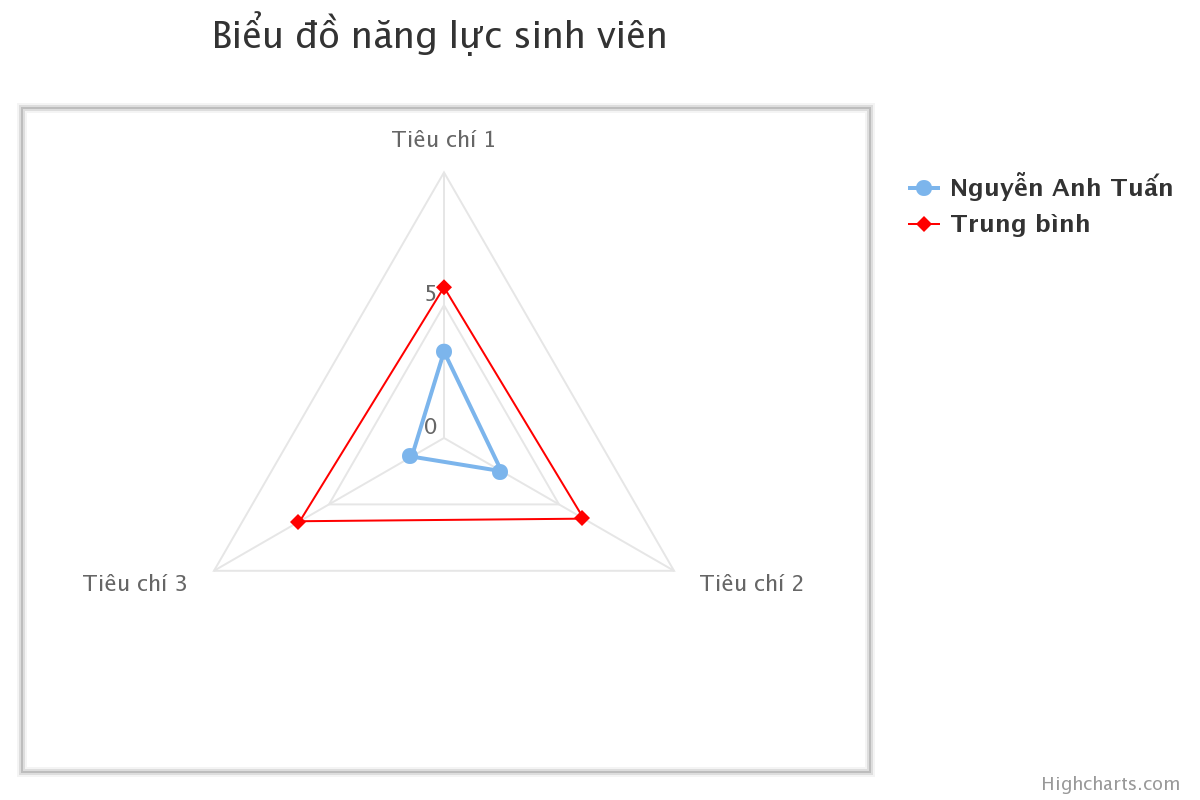
\includegraphics[width=0.8\linewidth]{img/22}
			\end{center}
			\caption{Giao diện biểu đồ mạng nhện}
			\label{refhinh70}
		\end{figure}
	\end{center}

	\begin{center}
		\begin{figure}[htp]
			\begin{center}
				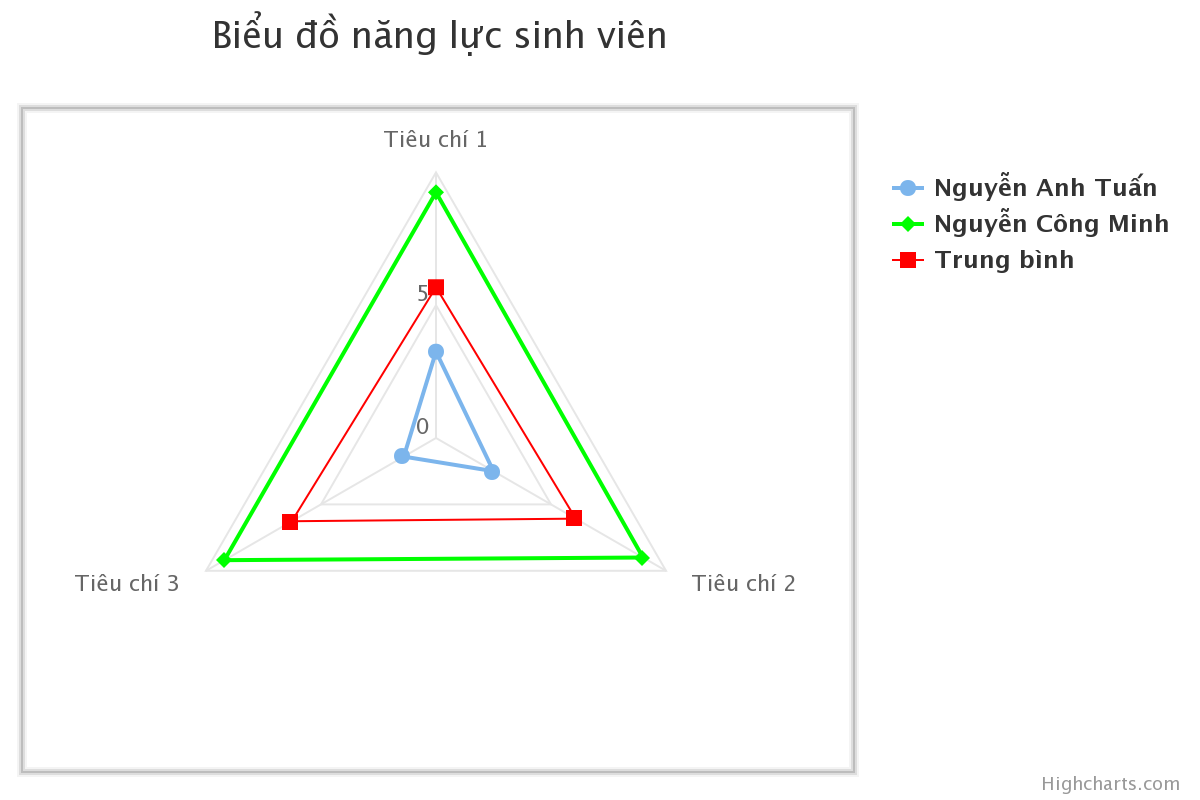
\includegraphics[width=0.8\linewidth]{img/25}
			\end{center}
			\caption{Biểu đồ so sánh 2 sinh viên}
			\label{refhinh71}
		\end{figure}
	\end{center}

	\item Thứ hai, chúng em đã thống kê được số lượt truy cập cũng như là không truy cập của sinh viên đối với một hạng mục cụ thể nào đó. Kết quả được hiển thị như hình sau
	
	\begin{center}
		\begin{figure}[htp]
			\begin{center}
				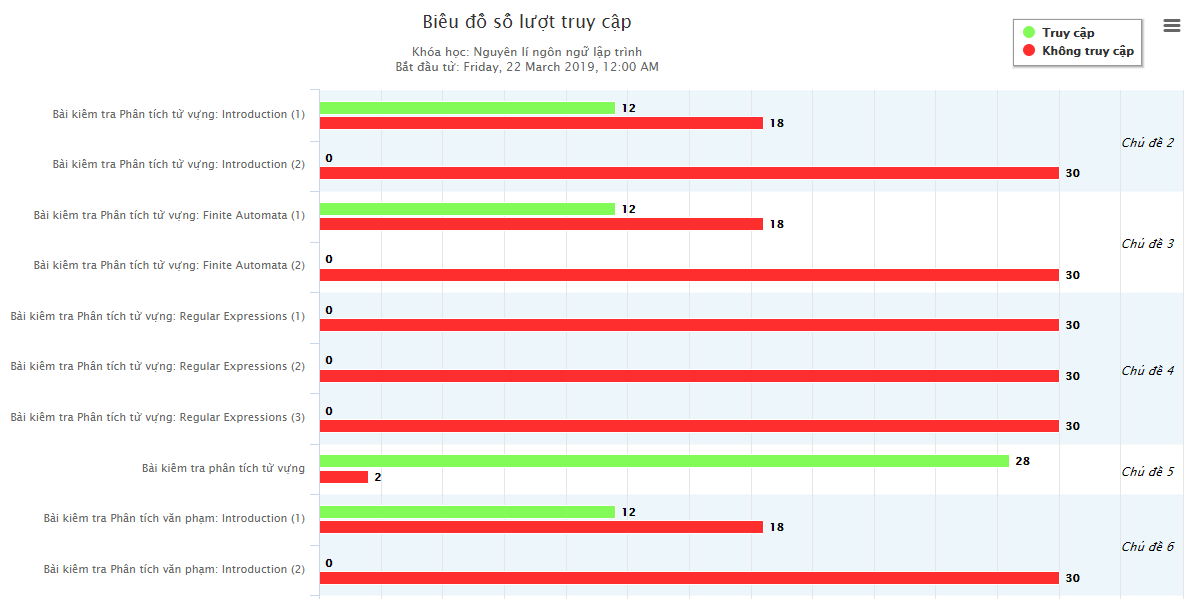
\includegraphics[width=1\linewidth]{img/27}
			\end{center}
			\caption{Biểu đồ cột ngang}
			\label{refhinh72}
		\end{figure}
	\end{center}

	\vskip 5cm
	\item Thứ ba, xây dựng thành công được chức năng nhằm đánh giá thái độ học tập của sinh viên dựa vào biểu đồ phân phối lượt truy cập của từng sinh viên.
	
	\begin{center}
		\begin{figure}[htp]
			\begin{center}
				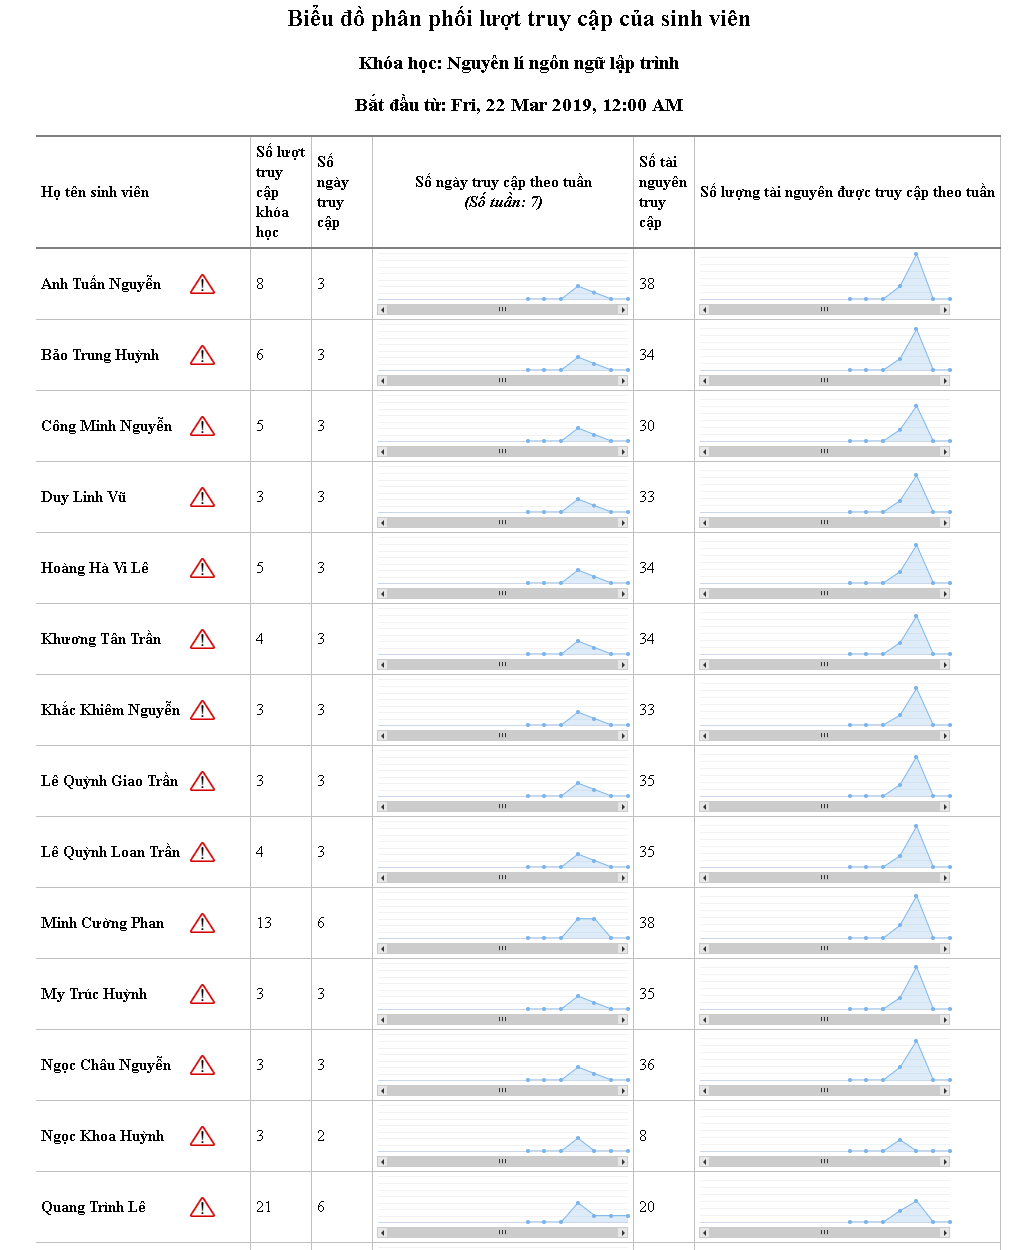
\includegraphics[width=0.8\linewidth]{img/29}
			\end{center}
			\caption{Biểu đồ phân phối lượt truy cập của SV}
			\label{refhinh73}
		\end{figure}
	\end{center}

	\begin{center}
		\begin{figure}[htp]
			\begin{center}
				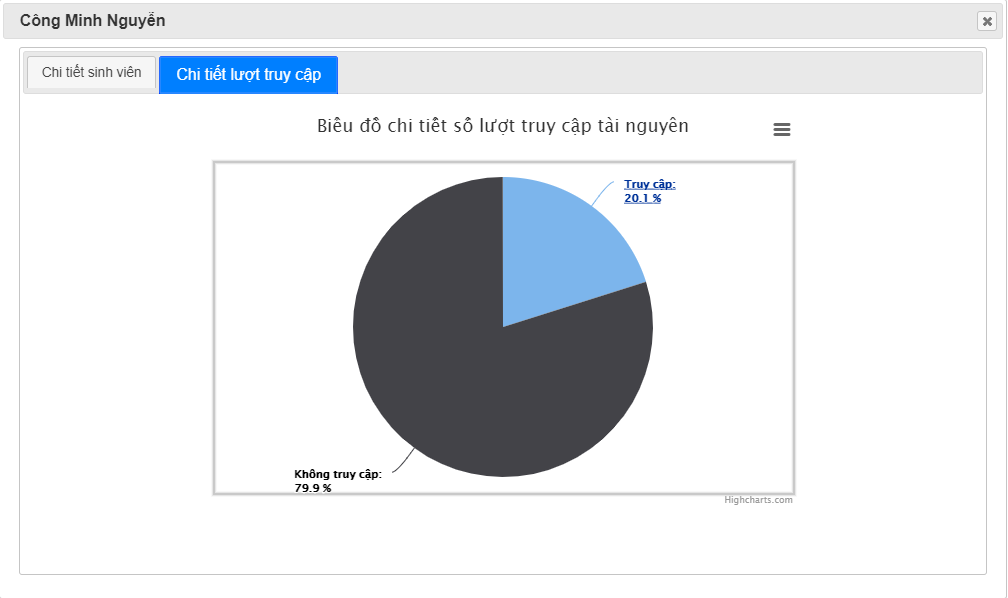
\includegraphics[width=0.6\linewidth]{img/41}
			\end{center}
			\caption{Biểu đồ thể hiện phần trăm truy cập}
			\label{refhinh74}
		\end{figure}
	\end{center}

	\vskip 5cm
	\item Chức năng cuối cùng mà nhóm xây dựng được cho giáo viên đó là bảng hỗ trợ cho giáo viên thêm tài liệu tham khảo.
	
	\begin{center}
		\begin{figure}[htp]
			\begin{center}
				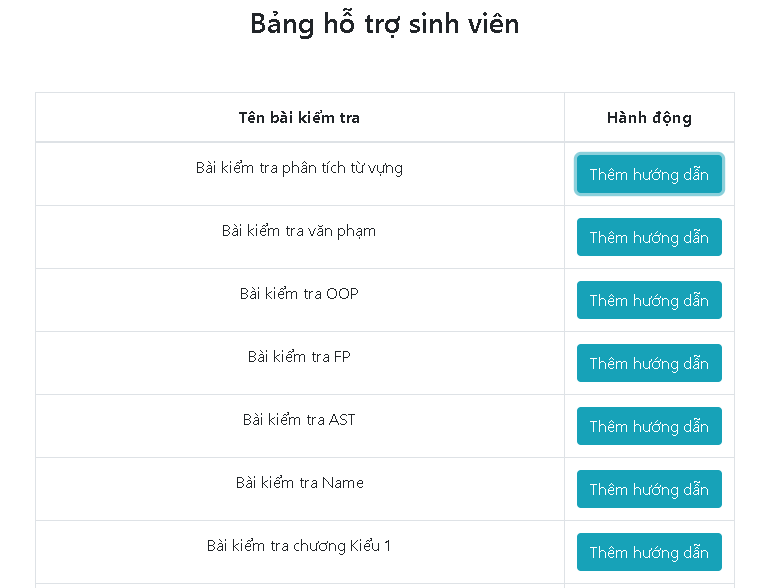
\includegraphics[width=0.6\linewidth]{img/30}
			\end{center}
			\caption{Chức năng cuối cùng dành cho GV}
			\label{refhinh75}
		\end{figure}
	\end{center}

	\begin{center}
		\begin{figure}[htp]
			\begin{center}
				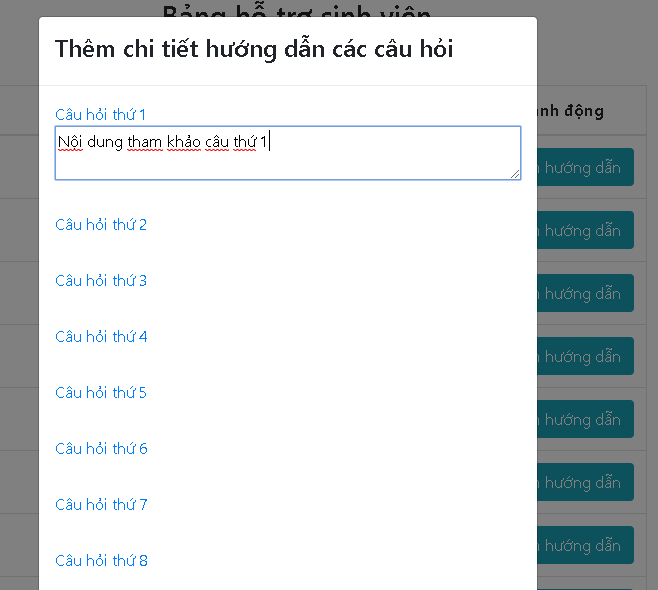
\includegraphics[width=0.6\linewidth]{img/31}
			\end{center}
			\caption{Chức năng cuối cùng dành cho GV}
			\label{refhinh76}
		\end{figure}
	\end{center}

\end{itemize}

\vskip 6cm
\subsection{Đối với HS, SV}

Đối với HS, SV nhóm đã xây dựng được một chức năng nhằm giúp cho HS, SV có thể tham khảo lại chi tiết bài kiểm tra mà mình đã làm ở lần cuối cùng.

\begin{center}
	\begin{figure}[htp]
		\begin{center}
			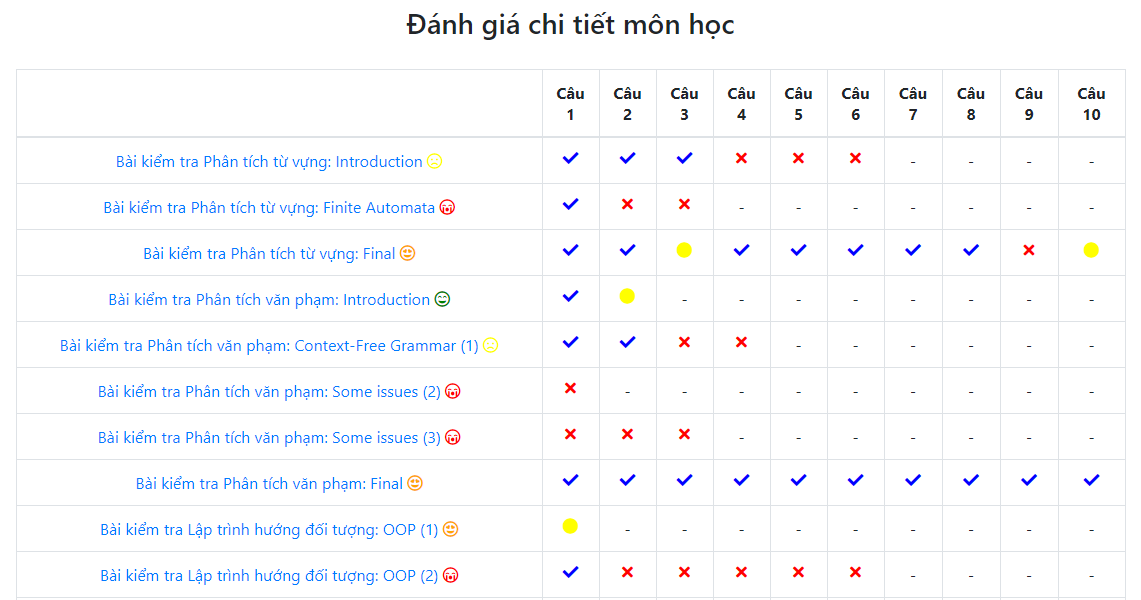
\includegraphics[width=1\linewidth]{img/33}
		\end{center}
		\caption{Bảng xem lại khóa học của sinh viên}
		\label{refhinh77}
	\end{figure}
\end{center}

Nội dung chi tiết của từng câu hỏi.

\begin{center}
	\begin{figure}[htp]
		\begin{center}
			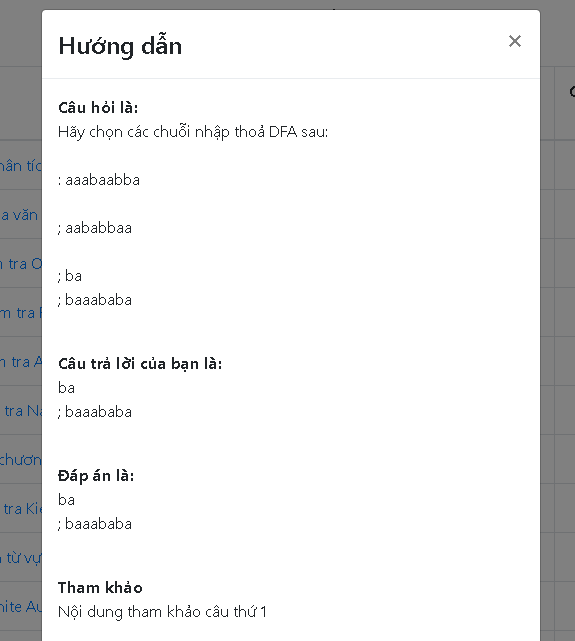
\includegraphics[width=0.5\linewidth]{img/34}
		\end{center}
		\caption{Nội dung chi tiết của từng câu hỏi}
		\label{refhinh78}
	\end{figure}
\end{center}
